\documentclass[12pt,fleqn,answers]{exam}
%\usepackage{pifont}
%\usepackage{dingbat,bbding}

\usepackage{amssymb}
\usepackage[intlimits]{amsmath}
\usepackage{epsfig}
\usepackage{upgreek}
\usepackage[super]{nth}
\usepackage[colorlinks=true,linkcolor=black,anchorcolor=black,citecolor=black,filecolor=black,menucolor=black,runcolor=black,urlcolor=black]{hyperref}
\usepackage[letterpaper, margin=0.75in]{geometry}
\addpoints
\boxedpoints
\pointsinmargin
\pointname{pts}
\usepackage{tikz}
\usepackage{tkz-euclide}
\usetikzlibrary{shapes.geometric}
\usetikzlibrary{calc}
\usepackage[final]{microtype}
\frenchspacing
\usepackage[american]{babel}
\usepackage[T1]{fontenc}
\usepackage[]{fourier}
\usepackage{isomath}
\usepackage{upgreek,amsmath}
\usepackage{amssymb}
\usepackage{graphicx}

\newcommand{\dotprod}{\, {\scriptzcriptztyle\stackrel{\bullet}{{}}}\,}

\newcommand{\reals}{\mathbf{R}}
\newcommand{\lub}{\mathrm{lub}} 
\newcommand{\glb}{\mathrm{glb}} 
\newcommand{\complex}{\mathbf{C}}
\newcommand{\dom}{\mbox{dom}}
\newcommand{\range}{\mbox{range}}
\newcommand{\cover}{{\mathcal C}}
\newcommand{\integers}{\mathbf{Z}}
\newcommand{\vi}{\, \mathbf{i}}
\newcommand{\vj}{\, \mathbf{j}}
\newcommand{\vk}{\, \mathbf{k}}
\newcommand{\bi}{\, \mathbf{i}}
\newcommand{\bj}{\, \mathbf{j}}
\newcommand{\bk}{\, \mathbf{k}}
\DeclareMathOperator{\Arg}{\mathrm{Arg}}
\DeclareMathOperator{\Ln}{\mathrm{Ln}}
\newcommand{\imag}{\, \mathrm{i}}

\usepackage{graphicx}
\usepackage{color}
%\shadedsolutions
%\definecolor{SolutionColor}{rgb}{1,0.72,0.46} %{0.8,0.9,1}
\newcommand\AM{\textsc{am}}
\newcommand\PM{\textsc{pm}}
     
\newcommand{\quiz}{5(a)}
\newcommand{\term}{Fall}
\newcommand{\due}{Tuesday 19 September 13:20}
\newcommand{\class}{MATH 202, Fall \the\year}
\begin{document}
\large
\vspace{0.1in}
\noindent\makebox[3.0truein][l]{\textbf{\class}}
\textbf{Name:} \hrulefill \\
\noindent \makebox[3.0truein][l]{\textbf{In class work week \quiz}}
\textbf{Row and Seat}:\hrulefill\\
\vspace{0.1in}


\noindent  In class work  \textbf{\quiz\/}  has questions \textbf{1} through  \textbf{\numquestions} \/ with a total of \textbf{\numpoints\/}  points.   
Turn in your work at the end of class  \emph{on paper}. This assignment is due \emph{\due}.

\vspace{0.1in}


\begin{questions} 

\question [2] Use IBP to find an antiderivative of the inverse cosine function;
that is find $\int \cos^{-1}(x) \, \mathrm{d} x$. To do the IBP,
integrate one and differentiate $\cos^{-1}(x)$.

\begin{solution}[2.8in] In tabular form, IBP gives

   \begin{equation*}
   \begin{array}{|c|c|c|} \hline 
        & \textbf{D} & \textbf{I}  \\ \hline 
         + &   \cos^{-1}(x) & 1 \\ \hline 
         - &  -\frac{1}{\sqrt{1-x^2}} & x  \\ \hline 
   \end{array}
\end{equation*}
So 
\begin{align*}
    \int \cos^{-1}(x) \, \mathrm{d} x 
       &= x \cos^{-1}(x) + 
             \int \frac{x}{\sqrt{1-x^2}} \, \mathrm{d} x, \\
       &= x \cos^{-1}(x) -\sqrt{1-x^2}.
\end{align*}
For $\int \frac{x}{\sqrt{1-x^2}} \, \mathrm{d} x$, let $z = 1-x^2$.
That gives $\int \frac{x}{\sqrt{1-x^2}} \, \mathrm{d} x = -\sqrt{1-x^2}$.

\end{solution}

\question [2] Find the area of the region $\{(x,y) | 0 \leq y \leq \cos^{-1}(x) 
\mbox{ and }  -1 \leq x \leq 1 \}$. A pretty good graph of this region 
is 

\begin{figure*}[h]
\begin{center}
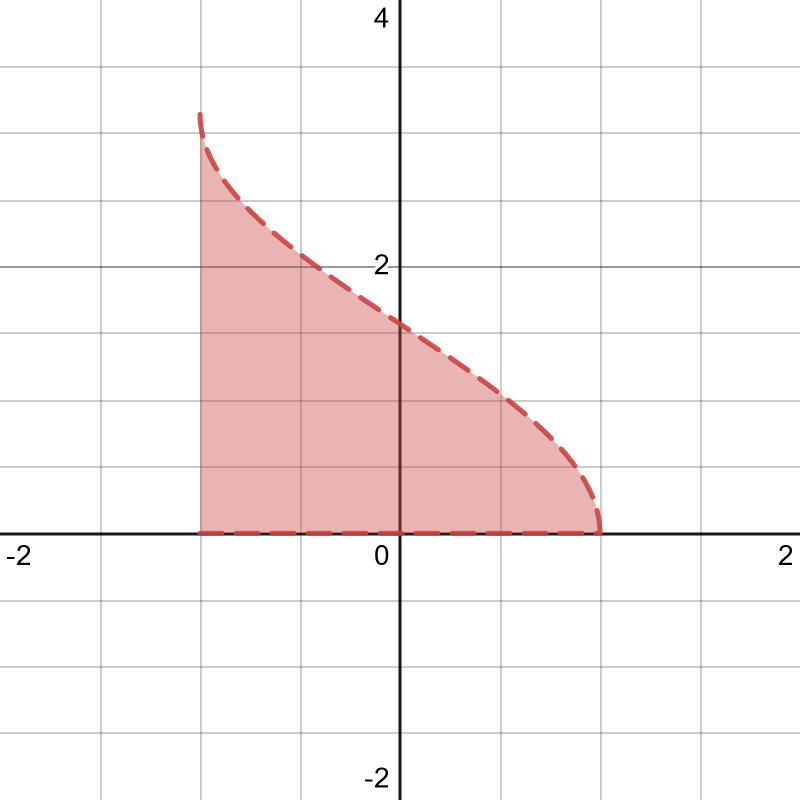
\includegraphics[scale=0.15]{desmos-graph(58).png}
\end{center}
\caption{A pretty good graph of $\{(x,y) | 0 \leq y \leq \cos^{-1}(x) 
\mbox{ and }  -1 \leq x \leq 1 \}$.}
\end{figure*}
\begin{solution}%[2.8in]

We have
\begin{equation*}
    \int_{-1}^1 \cos^{-1}(x) \, \mathrm{d} x = 
    \left.  x \cos^{-1}(x) -\sqrt{1-x^2} \right |_{x=-1}^{x=1}
    =\cos^{-1}(1) + \cos^{-1}(-1) = \uppi.
\end{equation*}
\end{solution}

%\newpage 

\question [2] Find the area of the region $\{(x,y) | \cos^{-1}(x) \leq y 
\leq \uppi \mbox{ and }  -1 \leq x \leq 1 \}$. Try doing this by
being clever. A pretty good graph of this region is 

\begin{figure*}[h]
    \begin{center}
    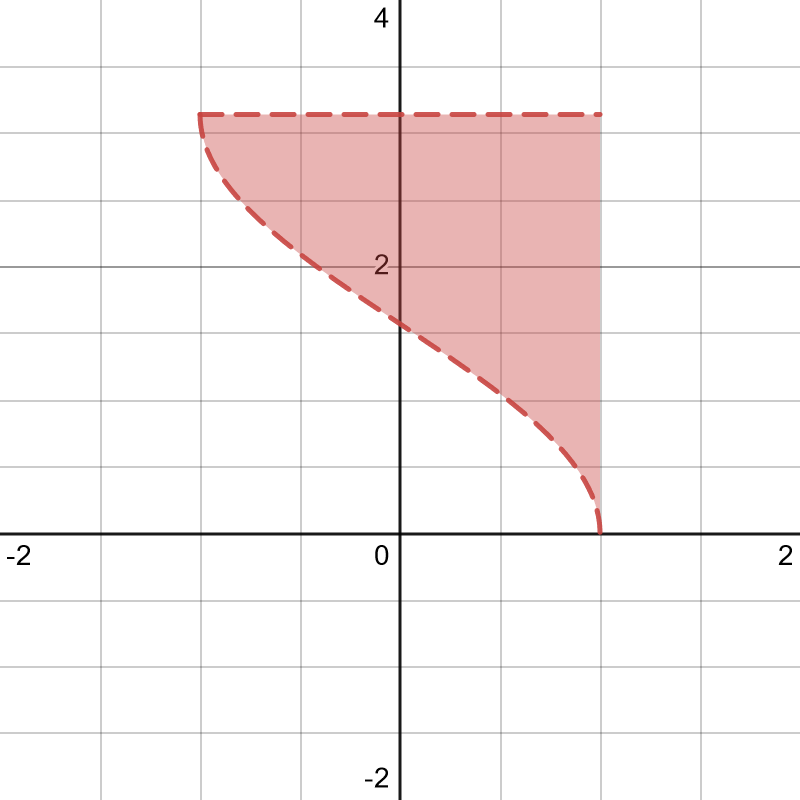
\includegraphics[scale=0.15]{desmos-graph(59).png}
    \end{center}
    \caption{A pretty good graph of $\{(x,y) | \cos^{-1}(x) \leq y 
    \leq \uppi \mbox{ and }  -1 \leq x \leq 1 \}$}
    \end{figure*}

    \begin{solution}[2.8in]
        To find the area of the given region, from the
         $2 \times \uppi $ rectangle with vertices
         $(-1,0), (1,0), (1, \uppi)$, and $(-1, \uppi)$, we 
         subtract the 
         area we found in the previous question. So this
         area is also $\uppi$.
    \end{solution}

\question [2] Use IBP to find $\int x (1-x) \sin (\uppi x) \, \mathrm{d} x$.
To do this, differentiate $x (1-x)$ and integrate $\sin (\uppi x)$.
If you enjoy doing more work than needed, expand the 
integrand as $\int x  \sin (\uppi x) \, \mathrm{d} x$ - 
$\int x^2 \sin (\uppi x) \, \mathrm{d} x$.

\begin{equation*}
    \begin{array}{|c|c|c|} \hline 
         & \textbf{D} & \textbf{I}  \\ \hline 
         + &  x - x^2 & \sin(\uppi x) \\ \hline 
         - &  1-2x  &  - \frac{1}{\uppi} \cos(\uppi x)  \\ \hline 
         + &  -2    &  \frac{1}{\uppi^2} \sin(\uppi x)  \\ \hline
         + &  0    &  -\frac{1}{\uppi^3} \cos(\uppi x)  \\ \hline
   \end{array}
\end{equation*}
So 
\begin{equation*}
    \int x  \sin (\uppi x) \, \mathrm{d} x = \frac{1}{\uppi^3} \left( {{\ensuremath{\pi} }^{2}}\, {{x}^{2}}- {{\ensuremath{\pi} }^{2}} x-2\right)  \cos{\left( \ensuremath{\pi}  x\right) }- \frac{1}{\uppi^2}   \left( 2 x-1\right)  \sin{\left( \ensuremath{\pi}  x\right) }.
\end{equation*}
\end{questions}

\end{document}

